\newpage
\def\thoigian{90}%--Thời gian
\de{Đề số 3}{Chương IV. Đường thẳng và mặt phẳng. Quan hệ song song trong không gian}

\begin{center}
	\textbf{PHẦN 1 - CÂU TRẮC NGHIỆM BỐN PHƯƠNG ÁN}
\end{center}
\Opensolutionfile{ans}[ans/ans-TN-ONTAPCHUONGIV-DE3]
\begin{ex}%[1H4H2-1]%[Dự án D đợt 4 - Nguyễn Hoàng Anh]%[Đề ôn tập Chương IV - Khối 11 - Đề số 3]
	Mệnh đề nào dưới đây đúng?
	\choice
	{Qua ba điểm phân biệt có duy nhất một mặt phẳng}
	{Qua hai điểm phân biệt có duy nhất một mặt phẳng}
	{\True Qua ba điểm không thẳng hàng có duy nhất một mặt phẳng}
	{Qua bốn điểm phân biệt có duy nhất một mặt phẳng}
	\loigiai{
		Qua ba điểm không thẳng hàng có duy nhất một mặt phẳng
	}
\end{ex}
\begin{ex}%[1H4N1-1]%[Dự án D đợt 4 - Nguyễn Hoàng Anh]%[Đề ôn tập Chương IV - Khối 11 - Đề số 3]
	Cho bốn điểm không đồng phẳng, ta có thể xác định được nhiều nhất bao nhiêu mặt phẳng phân biệt từ bốn điểm đã cho?
	\choice
	{$3$}
	{\True $4$}
	{$6$}
	{$2$}
	\loigiai{
		Cho bốn điểm không đồng phẳng, ta có thể xác định được nhiều nhất $4$ mặt phẳng phân biệt từ bốn điểm đã cho.
	}
\end{ex}
\begin{ex}%[1H4N2-1]%[Dự án D đợt 4 - Nguyễn Hoàng Anh]%[Đề ôn tập Chương IV - Khối 11 - Đề số 3]
	Cho tứ diện $ABCD$ có $M$, $N$ lần lượt là trung điểm của $AB$ và $CD$. Khi đó hai đường thẳng $AC$ và $MN$
	\choice
	{Trùng nhau}
	{Song song}
	{\True Chéo nhau}
	{Cắt nhau}
	\loigiai{
		\immini
		{Hai đường thẳng $AC$ và $MN$ chéo nhau.}
		{\begin{tikzpicture}[>=stealth,line join=round,line cap=round]
				\path (0,0)coordinate(B) (1,2.5)coordinate(A) (2,-1.5)coordinate(C) (3.5,0)coordinate(D) ;
				\coordinate (M) at ($(A)!0.5!(B)$);
				\coordinate (N) at ($(C)!0.5!(D)$);
				\draw (A)--(B)--(C)--(D)--(A)--(C);
				\draw[dashed] (B)--(D)  (M)--(N);
				\foreach \diem/\vitrin in {A/above,B/left,C/below left,D/right,M/left,N/right}	\fill (\diem)circle(1.5pt)node[\vitrin]{$\diem$};
		\end{tikzpicture}}
	}
\end{ex}

\begin{ex}%[1H4N2-2]%[Dự án D đợt 4 - Nguyễn Hoàng Anh]%[Đề ôn tập Chương IV - Khối 11 - Đề số 3]
	Cho hình chóp $S.ABCD$ có đáy $ABCD$ là hình bình hành tâm $O$. Gọi $M$, $N$ lần lượt là trung điểm của $SA$ và $SB$. Trong các khẳng định sau, khẳng định nào \textbf{sai}?
	\begin{center}
		\begin{tikzpicture}[>=stealth,line join=round,line cap=round,font=\footnotesize,scale=1]
			\path 
			(2.4,-1) coordinate (C)
			(0,0) coordinate (A)
			(3.4,0) coordinate (B)
			($(A)-(B)+(C)$) coordinate (D)
			(0.5,3) coordinate (S)
			($(S)!0.5!(A)$) coordinate (M)
			($(S)!0.5!(B)$) coordinate (N)
			($(C)!0.5!(A)$) coordinate (O);
			\draw (S)--(D)--(C)--(S)--(B)--(C) ;
			\draw[dashed] (S)--(A)--(C) (M)--(N)--(O)--(M) (A)--(D)--(B)--(A);
			\foreach \l/\g in {A/180,B/0,C/-45,D/-135,S/90,N/45,O/-90}
			\draw[fill=black] (\l) circle (1pt) +(\g:.3) node{$\l$};
			\draw[fill=black] (M) circle (1pt) +(30:.45) node{$M$};
		\end{tikzpicture}
	\end{center}
	\choice
	{$MN \parallel AB$}
	{$ON \parallel SD$}
	{\True $OM \parallel SB$}
	{$AD \parallel BC$}
	\loigiai{
		Vì $ABCD$ là hình bình hành tâm $O$ nên $O$ là trung điểm của $AC$ và $BD$.\\
		Mà $M$ là trung điểm của $SA$ nên $OM$ là đường trung bình của $\triangle SAC$ do đó $OM \parallel SC$.\\
		Vậy khẳng định $OM \parallel SB$ là sai.
	}
\end{ex}
\begin{ex}%[1H4B3-2]%[Dự án D đợt 4 - Nguyễn Hoàng Anh]%[Đề ôn tập Chương IV - Khối 11 - Đề số 3]
	Cho hình chóp $S.ABCD$ có đáy $ABCD$ là hình bình hành. Gọi $M$, $N$, $K$ lần lượt là trung điểm các cạnh $AB$, $BC$, $SB$. Chọn khẳng định đúng trong các khẳng định dưới đây.
	\choice
	{$MK \parallel (SDN)$}
	{$KN \parallel (SBC)$}
	{$MN \parallel (SAD)$}
	{\True $KN \parallel (SDC)$}
	\loigiai{
		\immini{
			Vì $N$, $K$ lần lượt là trung điểm các cạnh $BC$, $SB$ nên $KN$ là đường trung bình của $\triangle SBC$.\\
			Suy ra $KN \parallel SC$.\\
			Ta có $\heva{&KN \not\subset (SDC)\\&KN \parallel SC \textrm{ (cmt)}\\&SC \subset (SDC)} \Rightarrow KN \parallel (SDC)$.
		}{
			\begin{tikzpicture}[>=stealth,line join=round,line cap=round,font=\footnotesize,scale=1]
				\path 
				(1,0) coordinate (A)
				(5,0) coordinate (B)
				(4,-1.5) coordinate (C)
				(0,-1.5) coordinate (D)
				(0.45,3.16) coordinate (S)
				($(A)!0.5!(B)$) coordinate (M)
				($(B)!0.5!(C)$) coordinate (N)
				($(S)!0.5!(B)$) coordinate (K);
				\draw (S)--(D)--(C)--(B)--(S)--(C) (K)--(N);
				\draw[dashed] (C)--(A)--(S) (B)--(A)--(D)--(B) (N)--(M)--(K);
				\foreach \l/\g in {S/90,A/180,B/0,C/-90,D/-90,N/-45,M/45,K/90}
				\draw[fill=black] (\l) circle (1pt) +(\g:.3) node{$\l$};
			\end{tikzpicture}
		}
	}
\end{ex}
\begin{ex}%[1H4H3-2]%[Dự án D đợt 4 - Nguyễn Hoàng Anh]%[Đề ôn tập Chương IV - Khối 11 - Đề số 3]
	Cho hình chóp tứ giác $S.A B C D$. Gọi $M$ và $N$ lần lượt là trung điểm của $S A$ và $S C$. Khẳng định nào sau đây \textbf{đúng}?
	\choice
	{$M N \parallel (S A B)$}
	{$M N \parallel (S C D)$}
	{\True $M N \parallel (A B C D)$}
	{$M N \parallel (S B C)$}
	\loigiai{
		\immini{
			Ta có $MN$ là đường trung bình tam giác $SAC$ nên $MN \parallel AC$. \\
			Mà $AC \subset (ABCD)$ và $MN \not\subset (ABCD)$ nên $MN \parallel (ABCD)$.}
		{
			\begin{tikzpicture}
				\def\a{3}
				\path 	(0:0) coordinate (A)
				++(0:\a) coordinate (D)
				++(-130:\a/2) coordinate (C)
				++(-165:2*\a/3) coordinate (B)
				($(A)+(70:\a)$) coordinate (S)
				(intersection of A--C and B--D) coordinate (O)
				($(S)!.5!(A)$)coordinate (M)
				($(S)!.5!(C)$)coordinate (N)
				;
				\draw[dashed,] (M)--(N) (A)--(C)	(A)--(D);
				\draw[] 			(A)--(B)--(C)--(D)
				(A)--(S)	(B)--(S)	(C)--(S)	(D)--(S);
				\foreach \x/\g in {A/180,B/-135,C/-45,D/0,S/90,M/180,N/0}
				\fill[black] 	(\x) circle (1pt)
				($(\g:3mm)+(\x)$) node {$\x$};	
			\end{tikzpicture}
		}
}\end{ex}
\begin{ex}%[1H4H4-2]%[Dự án D đợt 4 - Nguyễn Hoàng Anh]%[Đề ôn tập Chương IV - Khối 11 - Đề số 3]
	Cho tứ diện $A B C D$, gọi $G_1$, $G_2$, $G_3$ theo thứ tự là trọng tâm các tam giác $\triangle ABC$, $\triangle ACD$, $\triangle ABD$. Mặt phẳng $\left(G_1G_2G_3\right)$ song song với mặt phẳng nào trong các mặt phẳng sau đây?
	\choice
	{$(ACD)$}
	{$\left(BCG_2\right)$}
	{\True $(BCD)$}
	{$(ABC)$}
	\loigiai{
		\immini
		{Gọi $M$, $N$, $P$ lần lượt là trung điểm các cạnh $BC$, $CD$ và $DB$.\\
			$G_1$, $G_2$, $G_3$ theo thứ tự là trọng tâm các tam giác $\triangle ABC$, $\triangle ACD$, $\triangle ABD$ nên $\dfrac{AG_1}{AM}=\dfrac{AG_2}{AN}=\dfrac{AG_3}{AP}=\dfrac{2}{3}$.\\
			Do đó $G_1G_2\parallel MN$, $G_2G_3\parallel NP$.\\
			Ta có $\heva{& G_1G_2 \not\subset (BCD) \\ & G_1G_2\parallel MN\\&MN\subset (BCD) }\Rightarrow G_1G_2 \parallel(BCD)$.\\
			Tương tự $\heva{& G_2G_3 \not\subset (BCD) \\ & G_2G_3\parallel NP\\&NP\subset (BCD) }\Rightarrow G_2G_3 \parallel(BCD)$.\\
			Mà	$G_1G_2, G_2G_3\subset (G_1G_2G_3)$ và $G_1G_2\cap G_2G_3=G_2$ nên suy ra $\left(G_1G_2G_3\right)\parallel (BCD)$.
		}
		{
			\begin{tikzpicture}[line join=round, line cap=round,,scale=0.7]
				\def\h{5}
				\path
				(0,0) coordinate (B)
				(6,0) coordinate (D)
				(2,-2) coordinate (C)
				;
				\path ($(1,\h)+(B)$) coordinate (A)
				(barycentric cs:A=1,B=1,C=1)coordinate(G_1)
				(barycentric cs:A=1,C=1,D=1)coordinate(G_2)
				(barycentric cs:A=1,D=1,B=1)coordinate(G_3)
				(barycentric cs:B=1,C=1)coordinate(M)
				(barycentric cs:C=1,D=1)coordinate(N)
				(barycentric cs:D=1,B=1)coordinate(P);
				\draw[dashed] (B)--(D) (A)--(P) (M)--(N)--(P)--cycle (G_1)--(G_2)--(G_3)--cycle;
				\draw (A)--(B)--(C)--(D)--cycle (A)--(C) (A)--(M) (A)--(N); 
				\foreach \i/\j in {B/180,C/-120,D/0,A/90,M/180,N/0,P/60,G_1/160,G_2/30,G_3/160}\fill  (\i) circle(1.5pt) ($(\i) + (\j:5mm)$)node{$\i$};
			\end{tikzpicture}	
		}	
	}
\end{ex}
\begin{ex}%[1H4N3-2]%[Dự án D đợt 4 - Nguyễn Hoàng Anh]%[Đề ôn tập Chương IV - Khối 11 - Đề số 3]
	\immini[thm]{
		Cho hình chóp tứ giác $S.ABCD$. Gọi $I$, $J$ lần lượt là trung điểm của $SB$ và $SD$. Mệnh đề nào sau đây đúng?
		\choice
		{$IJ \parallel (SBC)$}
		{$IJ \parallel (SBD)$}
		{\True $IJ \parallel (ABCD)$}
		{$IJ \parallel (SAB)$}
	}{
		\begin{tikzpicture}[>=stealth,line join=round,line cap=round,font=\footnotesize,scale=0.8]
			\path
			(1.3,2) coordinate (S)
			(3.4,0) coordinate (A)
			(2.6,-1) coordinate (B)
			(0.8,-1.4) coordinate (C)
			(0,0) coordinate (D)
			($(S)!0.5!(B)$) coordinate (I)
			($(S)!0.5!(D)$) coordinate (J)
			;
			\draw (C)--(D)--(S)--(C)--(B)--(S)--(A)--(B);
			\draw[dashed] (A)--(D)--(B) (I)--(J);
			\foreach \d/\g in {A/0,B/-55,C/-90,D/-135,S/90,J/160,I/10} \fill (\d)node[shift={(\g:0.3)}]{$\d$} circle(1pt);
		\end{tikzpicture}
	}
	\loigiai{
		Xét $\triangle SBD$ có $I$, $J$ lần lượt là trung điểm của $SB$ và $SD$ nên $IJ$ là đường trung bình của $\triangle SBD$.\\
		Do đó $IJ \parallel BD$, mà $BD \subset (ABCD)$ nên $IJ \parallel (ABCD)$.
	}
\end{ex}
\begin{ex}%[1H4H3-2]%[Dự án D đợt 4 - Nguyễn Hoàng Anh]%[Đề ôn tập Chương IV - Khối 11 - Đề số 3]
	Cho hình chóp $S.ABCD$ có đáy là hình bình hành tâm $O$. Gọi $M$ là trung điểm của $SA$. Đường thẳng $OM$ song song với mặt phẳng nào sau đây? 
	\choice
	{$(SBD)$}
	{$(ABCD)$}
	{\True $(SCD)$}
	{$(SAB)$}
	\loigiai{
		\immini
		{Ta có $OM\parallel SC$ và $SC\subset (SCD)$ suy ra $OM\parallel (SCD)$.}
		{\begin{tikzpicture}[>=stealth,line join=round,line cap=round, font=\footnotesize, scale=.8]
				\path
				(0,0) coordinate (A)
				(7,0) coordinate (B)
				(10,2) coordinate (C)
				(3,2) coordinate (D)
				(4,8) coordinate (S)
				($(S)!1/2!(A)$) coordinate (M)
				($(A)!1/2!(C)$) coordinate (O)
				;
				\draw (A)--(B)--(C)--(S)--(A) (S)--(B);
				\draw[dashed] (A)--(D)--(C) (S)--(D)--(B) (A)--(C) (O)--(M);
				\foreach \x/\g in {A/-120,B/-60,C/90,D/130,S/90,M/160,O/-90}\fill (\x) circle (1.5pt)+(\g:3mm) node{$\x$};
		\end{tikzpicture}}
	}
\end{ex}

\begin{ex}%[1H4H4-2]%[Dự án D đợt 4 - Nguyễn Hoàng Anh]%[Đề ôn tập Chương IV - Khối 11 - Đề số 3]
	Cho hình hộp $A B C D. A'B'C'D'$. Mặt phẳng $\left(A B'D'\right)$ song song với mặt phẳng nào trong các mặt phẳng sau đây?
	\choice
	{\True $\left(B C'D\right)$}
	{$\left(B C A'\right)$}
	{$\left(B D A'\right)$}
	{$\left(A'C'C\right)$}
	\loigiai{
		\immini{
			Ta có $(AB'D') \parallel (BC'D)$.}
		{
			\begin{tikzpicture}
				\def\a{3}
				\def\b{2}
				\def\h{3}
				\path 	(0:0) coordinate (A)
				++(0:\a) coordinate (D)
				++(-130:\b) coordinate (C)
				($(A)+(C)-(D)$) coordinate (B)
				($(A)+(80:\h)$) coordinate (A')
				($(B)+(80:\h)$) coordinate (B')
				($(C)+(80:\h)$) coordinate (C')
				($(D)+(80:\h)$) coordinate (D');
				\draw[dashed,] 	(B)--(A)--(D)	(A)--(A') (B')--(A)--(D') (B)--(D);
				\draw[] (B')--(D')	(C)--(C') 	(D)--(D') 	(B)--(B')	(C)--(C')
				(B)--(C)--(D) 
				(A')--(B')--(C')--(D')--cycle (B)--(C')--(D);
				\foreach \x/\g in {A/180,B/180,C/0,D/0,A'/180,B'/180,C'/0,D'/0}
				\fill[black] 	(\x) circle (1pt)
				($(\g:4mm)+(\x)$) node {$\x$};	
			\end{tikzpicture}	
		}
}\end{ex}
\begin{ex}%[1H4H4-2]%[Dự án D đợt 4 - Nguyễn Hoàng Anh]%[Đề ôn tập Chương IV - Khối 11 - Đề số 3]
	\immini{
		Cho hình chóp $S. ABCD$ có đáy $ABCD$ là hình bình hành tâm $O$. Gọi $M$, $N$, $P$ theo thứ tự là trung điểm của $SA$, $SD$ và $AB$. Khẳng định nào sau đây đúng?
		\choice
		{$(MOP) \parallel (SAB)$}
		{$(MON) \parallel (SCD)$}
		{$(MOP) \parallel (SAD)$}
		{\True $(MON) \parallel (SBC)$}
	}
	{
		\begin{tikzpicture}[line join=round, line cap=round,]
			\coordinate (A) at (0,0);
			\coordinate (B) at (2,-2);
			\coordinate (D) at (4,0);
			\coordinate (C) at ($(B)+(D)-(A)$);
			\coordinate (O) at ($(A)!0.5!(C)$);
			\coordinate (S) at ($(O)+(0,5)$);
			\draw(S)--(A) (S)--(B) (S)--(C) (A)--(B) (B)--(C);
			\draw[dashed,thin](A)--(C) (A)--(D) (C)--(D) (S)--(D) (S)--(O) (B)--(D);
			\path
			($(S)!0.5!(A)$) coordinate (M)
			($(S)!0.5!(D)$) coordinate (N)
			($(B)!0.5!(A)$) coordinate (P)
			;
			\draw[dashed, thin]
			(M)--(N)--(O)--cycle
			(O)--(P)
			;
			\draw (M)--(P);
			\foreach \i/\g in {S/90,A/180,B/-90,C/-90,D/0,O/-90, M/180, N/0, P/180}{\draw[fill=black](\i) circle (0.5pt) ($(\i)+(\g:3mm)$) node[scale=0.8]{$\i$};}
		\end{tikzpicture}
	}
	\loigiai{
		\begin{itemize}
			\item $(MOP) \cap (SAB) = MP$ nên $(MON) \nparallel (SAB)$.
			\item $(MON)$ và $(SCD)$ có điểm chung là $N$ nên $(MON) \nparallel (SCD)$.
			\item $(MOP)$ và $(SAD)$ có điểm chung là $M$ nên $(MOP) \nparallel (SAD)$.
			\item $\heva{& MN \parallel BC \\ & NO \parallel SB} \Leftrightarrow (MON) \parallel (SBC)$.
		\end{itemize}
	}
\end{ex}
\begin{ex}%[1H4H4-2]%[Dự án D đợt 4 - Nguyễn Hoàng Anh]%[Đề ôn tập Chương IV - Khối 11 - Đề số 3]
	\immini{Cho hình chóp tứ giác $S.ABCD$. Gọi $M$, $N$, $P$ lần lượt là trung điểm các cạnh $SA$, $AB$ và $AD$ \textit{(tham khảo hình vẽ)}. Mặt phẳng $(MNP)$ song song với mặt phẳng nào dưới đây?
		\choice
		{$(SBC)$}
		{\True $(SBD)$}
		{$(ABCD)$}
		{$(SCD)$}}
	{\begin{tikzpicture}[scale=0.8, font=\footnotesize,line join=round, line cap=round, >=stealth]
			\coordinate (A) at (0,0);
			\coordinate (B) at (1.2,-1.8);
			\coordinate (D) at (5,0);
			\coordinate (C) at (4,-2.0);
			\coordinate (S) at ($(A)+(2,3)$);
			\coordinate (M) at ($(S)!0.5!(A)$);
			\coordinate (N) at ($(B)!0.5!(A)$);
			\coordinate (P) at ($(D)!0.5!(A)$);
			\foreach \i in {A,B,C,D}{\draw (S)--(\i);}
			\draw (A)--(B)--(C)--(D) (M)--(N);
			\draw[dashed,thin] (A)--(D) (M)--(P)--(N);
			\foreach \i/\g in {S/90,A/180,B/-90,C/-90,D/0,M/135,N/-135,P/45}{\draw[fill=black](\i) circle (1.5pt) ($(\i)+(\g:3mm)$) node[scale=1]{$\i$};}
	\end{tikzpicture}}
	\loigiai{
		\immini{Ta có $\heva{&MN\parallel SB \\&NP\parallel BD\\&MN,NP\subset (MNP)\\& SB,BD \subset (SBD)}\Rightarrow (MNP) \parallel (SBD)$.}
		{\begin{tikzpicture}[scale=0.8, font=\footnotesize,line join=round, line cap=round, >=stealth]
				\coordinate (A) at (0,0);
				\coordinate (B) at (1.2,-1.8);
				\coordinate (D) at (5,0);
				\coordinate (C) at (4,-2.0);
				\coordinate (S) at ($(A)+(2,3)$);
				\coordinate (M) at ($(S)!0.5!(A)$);
				\coordinate (N) at ($(B)!0.5!(A)$);
				\coordinate (P) at ($(D)!0.5!(A)$);
				\foreach \i in {A,B,C,D}{\draw (S)--(\i);}
				\draw (A)--(B)--(C)--(D) (M)--(N);
				\draw[dashed,thin] (A)--(D) (M)--(P)--(N) (B)--(D);
				\foreach \i/\g in {S/90,A/180,B/-90,C/-90,D/0,M/135,N/-135,P/45}{\draw[fill=black](\i) circle (1.5pt) ($(\i)+(\g:3mm)$) node[scale=1]{$\i$};}
		\end{tikzpicture}}
	}
\end{ex}
\Closesolutionfile{ans}
%\begin{center}
%	\textbf{ĐÁP ÁN}
%	\inputansbox{10}{ans/ans}	
%\end{center}
\begin{center}
	\textbf{PHẦN 2 - CÂU TRẮC NGHIỆM ĐÚNG SAI}
\end{center}
\Opensolutionfile{ans}[ans/answer-DS-ONTAPCHUONGIV-DE3]
\begin{ex}%[1H4V4-6]%[Dự án D đợt 4 - Nguyễn Hoàng Anh]%[Đề ôn tập Chương IV - Khối 11 - Đề số 3]
	Cho hình chóp $S.ABCD$ có đáy $ABCD$ là hình thang có đáy lớn $AB$ và $AB=2 CD$. Gọi $E$ là trung điểm $BD, M$ là trung điểm $SB$.
	\choiceTF
	{\True $CM$ song song mặt phẳng $(SAD)$}
	{\True Giao điểm của $SA$ với $(DCM)$ là trung điểm của $SA$}
	{Giao tuyến của $(SAD)$ và $(SBC)$ là đường thẳng qua $S$ và song song $AD$}
	{\True Mặt phẳng $(CEM)$ song song mặt phẵng $(SAD)$}
	\loigiai{
		\begin{center}
			\begin{tikzpicture}[
				>=stealth, line join=round, line cap=round, 
				scale=.8,
				font=\footnotesize,
				declare function={r=3; a=75;}]
				% ve diem
				\path 
				(0,0) coordinate (A)
				($ (A)+(0:10) $) coordinate (B)
				($ (A)+(-70:3) $) coordinate (D)
				($ (D)+(0:5) $) coordinate (C)
				($ (A)+(75:6) $) coordinate (S)
				($(S)!.5!(B)$) coordinate (M)
				($(S)!.5!(A)$) coordinate (N)
				($(B)!.5!(D)$) coordinate (E)
				($(B)!.5!(A)$) coordinate (K)
				($(D)!-1!(A)$) coordinate (F)
				;
				\foreach \x/\g in {A/150, B/30, C/-45, D/180, S/90, E/-60, M/45, N/135, F/-120, K/135}{
					\draw[fill=black] (\x) circle (1.5pt)+(\g:.4) node{$\x$};}
				\draw[] 
				(M)--(C)--(S)
				(C)--(B)--(S)
				(C)--(F)--(S)--(A)--(F)
				(N)--(D)--(S)
				;
				\draw[dotted] 
				(B)--(D)--(C)--(A)--(B)
				(C)--(K)--(M)--(D)
				(E)--(M)--(N)
				;
				\foreach \a/\b/\c in {}	{
					\draw pic [draw=black,angle radius = 10] {right angle = \a--\b--\c};
				}
			\end{tikzpicture}
		\end{center}
		\begin{itemchoice}
			\itemch \textbf{Đúng}. Gọi $N$ là trung điểm của $SA$.\\
			Dễ thấy $MN = DC = \dfrac{AB}{2}$ và $MN \parallel DC \left(\parallel AB\right)$ nên $CDNM$ là hình bình hành.\\
			Khi đó, $CM \parallel DN $ với $DN \subset (SAD)$ nên $CM \parallel (SAD)$.
			
			\itemch \textbf{Đúng}. Do $CDNM$ là hình bình hành nên $N \in (DCM)$.\\
			Mà $N$ là trung điểm của $SA$ nên giao điểm của $SA$ với $(DCM)$ là trung điểm của $SA$.
			
			\itemch \textbf{Sai}. Trong mặt phẳng $(ABCD)$, gọi $F$ là giao điểm của $AD$ và $BC$.\\
			Khi đó, $SF$ là giao tuyến của $(SAD)$ và $(SBC)$.\\
			Ta thấy $SF$ cắt $AD$ tại $F$ nên khẳng định này là \textbf{sai}.
			
			\itemch \textbf{Đúng}. Gọi $K$ là trung điểm của $AB$ thì $CDKB$ và $CDAK$ là các hình bình hành.\\
			Do đó, trung điểm $E$ của $BD$ cũng là trung điểm của $CK$.\\
			Khi đó, mặt phẳng $(CEM)$ có chứa hai đường thẳng cắt nhau là $CM$ và $CK$ đều song song với mặt phẳng $(SAD)$ nên $(CEM) \parallel (SAD)$.
		\end{itemchoice}
	}
\end{ex} 
\begin{ex}%[1H4H3-2]%[Dự án D đợt 4 - Nguyễn Hoàng Anh]%[Đề ôn tập Chương IV - Khối 11 - Đề số 3]
	Cho hai hình bình hành $ABCD$ và $ABEF$ không cùng nằm trong một mặt phẳng và có tâm lần lượt $O$ và $O'$. Gọi $M$, $N$ theo thứ tự là hai điểm trên các cạnh $AE$, $BD$ sao cho $AM=\dfrac{1}{3}AE$, $BN=\dfrac{1}{3}BD$ (tham khảo hình vẽ).
	\begin{center}
		\begin{tikzpicture}[scale=0.7, font=\footnotesize, line join=round, line cap=round, >=stealth]
			\coordinate (A) at (0,0);
			\coordinate (B) at (5,0);
			\coordinate (D) at (-2,-2);
			\coordinate (C) at ($(B)+(D)-(A)$);
			\coordinate (O) at ($(A)!0.5!(C)$);
			\coordinate (F) at ($(O)+(-3,4)$);
			\coordinate (E) at ($(B)+(F)-(A)$);
			\coordinate (O') at ($(A)!0.5!(E)$);
			\coordinate (M) at ($(A)!1/3!(E)$);
			\coordinate (N) at ($(B)!1/3!(D)$);
			\draw (F)--(D)--(C)--(B)--(E)--(F) (C)--(E) (C)--(F);
			\draw[dashed](A)--(B)--(F)--(A)--(D)--(B) (E)--(A)--(C) (O)--(O') (M)--(N);
			\foreach \i/\g in {F/90,A/180,B/0,C/-90,D/-90,O/-90,E/90,O'/90,M/100,N/-120}{\draw[fill=black](\i) circle (1.5pt) ($(\i)+(\g:3mm)$) node[scale=1]{$\i$};}
		\end{tikzpicture}
	\end{center}
	\choiceTF
	{\True $OO'$ song song với mặt phẳng $(ADF)$}
	{$OO'$ cắt mặt phẳng $(BCE)$}
	{\True $MN$ song song $CF$}
	{\True $MN$ song song với mặt phẳng $(CDFE)$}
	\loigiai{
		Gọi $I$ là trung điểm của $AB$.
		\begin{center}
			\begin{tikzpicture}[scale=0.7, font=\footnotesize, line join=round, line cap=round, >=stealth]
				\coordinate (A) at (0,0);
				\coordinate (B) at (5,0);
				\coordinate (D) at (-2,-2);
				\coordinate (C) at ($(B)+(D)-(A)$);
				\coordinate (O) at ($(A)!0.5!(C)$);
				\coordinate (F) at ($(O)+(-3,4)$);
				\coordinate (E) at ($(B)+(F)-(A)$);
				\coordinate (O') at ($(A)!0.5!(E)$);
				\coordinate (M) at ($(A)!1/3!(E)$);
				\coordinate (N) at ($(B)!1/3!(D)$);
				\coordinate (I) at ($(A)!0.5!(B)$);
				\draw (F)--(D)--(C)--(B)--(E)--(F) (C)--(E) (C)--(F);
				\draw[dashed](A)--(B)--(F)--(A)--(D)--(B) (E)--(A)--(C) (O)--(O') (M)--(N) (C)--(I)--(F);
				\foreach \i/\g in {F/90,A/180,B/0,C/-90,D/-90,O/-90,E/90,O'/90,M/100,N/-120,I/90}{\draw[fill=black](\i) circle (1.5pt) ($(\i)+(\g:3mm)$) node[scale=1]{$\i$};}
			\end{tikzpicture}
		\end{center}
		\begin{itemchoice}
			\itemch \textbf{Đúng}.\\
			Vì $OO'$ là đường trung bình tam giác $BDF$ nên $OO'\parallel DF\Rightarrow OO'\parallel (ADF)$.
			\itemch \textbf{Sai}.\\
			Vì $OO'$ là đường trung bình tam giác $ACE$ nên $OO'\parallel CE\Rightarrow OO'\parallel (BCE)$.
			\itemch \textbf{Đúng}.\\
			Theo giả thiết $BN=\dfrac{1}{3}BD$ và $O$ là trung điểm của $BD$ nên $BN=\dfrac{2}{3}BO$.\\
			Mặt khác $BO$ là đường trung tuyến tam giác $ABC\Rightarrow N$ là trọng tâm tam giác $ABC$.\\
			Tương tự $M$ là trọng tâm tam giác $ABF$.\\
			Xét tam giác $ICF$ có $\dfrac{IM}{IF}=\dfrac{IN}{IC}=\dfrac{1}{3}\Rightarrow \dfrac{MN}{CF}=\dfrac{1}{3}\Rightarrow MN\parallel CF$.
			\itemch \textbf{Đúng}.\\
			Vì $MN\parallel CF$ nên $MN\parallel (CDFE)$.
		\end{itemchoice}
	}
\end{ex}
\Closesolutionfile{ans}
%\inputansbox[2]{2}{ans/answer.tex}
\begin{center}
\textbf{PHẦN 3 - CÂU TRẮC NGHIỆM TRẢ LỜI NGẮN}
\end{center}
\setcounter{ex}{0}
\Opensolutionfile{ans}[ans-KQ-ONTAPCHUONGIV-DE3]
\begin{ex}%[1H4H3-4]%[Dự án D đợt 4 - Nguyễn Hoàng Anh]%[Đề ôn tập Chương IV - Khối 11 - Đề số 3]
	Cho hình chóp $S. ABC$, gọi $G$ là trọng tâm tam giác $SBC$, $M$ là trung điểm của $AC$. Giả sử $BM$ cắt mặt phẳng $(SAG)$ tại $H$ và $HM=k HB$. Tìm $k$.
	
	\shortans{$0{,}5$}
	\loigiai{
		\immini{
			Trong $(SBC)$, gọi $N=SG\cap BC$, khi đó $N$ là trung điểm $BC$.\\
			Trong $(ABC)$, gọi $H=AN\cap MB$.\\
			Khi đó $\heva{& H\in MB\\ & H\in AN\subset (SAG)} \Rightarrow H=MB\cap (SAG)$.\\
			Vì $BM$, $AN$ là các đường trung tuyến nên $H$ là trọng tâm $\triangle ABC$.\\
			Do đó $\dfrac{HM}{HB}=\dfrac{1}{2}$ hay $HM=\dfrac{1}{2}HB$.\\
			Vậy $k=\dfrac{1}{2}=0{,}5$.	
		}{
			\begin{tikzpicture}[scale=0.9,font=\footnotesize,line join=round,line cap=round,>=stealth]
				
				\def\a{5}
				\def\h{4.5}
				\path 	(0:0) coordinate (A)
				++(0:\a) coordinate (B)
				++(-150:4*\a/5) coordinate (C)
				($(A)!0.5!(C)$) coordinate (M)
				($(B)!0.5!(C)$) coordinate (N)
				($(B)!2/3!(M)$) coordinate (H)
				($(H)+(90:\h)$) coordinate (S)
				($(S)!2/3!(N)$) coordinate (G)
				;
				\draw (C)--(A) (C)--(B) (S)--(N)
				(A)--(S)	(B)--(S)	(C)--(S);
				\draw[dashed] (A)--(B) (S)--(H) 	(G)--(A)--(N) (B)--(M);
				\foreach \x / \goc in {A/180,B/0,C/-135,H/-90,M/180,S/90,N/-60,G/45}
				\fill (\x) circle (1pt)
				($(\x)+(\goc:3mm)$) node {$\x$};
			\end{tikzpicture}
		}
	}
\end{ex}
\begin{ex}%[1H4H2-2]%[Dự án D đợt 4 - Nguyễn Hoàng Anh]%[Đề ôn tập Chương IV - Khối 11 - Đề số 3]
	Cho hình chóp $S.ABCD$, đáy $ABCD$ là hình bình hành, tam giác $SAC$ là tam giác đều cạnh $5$. Gọi $H$ là trung điểm $SD$, $K$ là điểm thuộc $BD$ sao cho $BD=4KD$. Tính độ dài đoạn thẳng $HK$ \textit{(kết quả làm tròn đến hàng phần chục)}.
	\shortans{$2{,}2$}
	\loigiai{\immini{
			Trong $(ABCD)$, gọi $O=AC\cap BD$.\\
			Vì $ABCD$ là hình bình hành nên $O$ là trung điểm của $AC$, $BD$.\\
			Ta có $\triangle ABC$ đều có cạnh bằng $5$ và $SO$ là trung tuyến của $\triangle ABC$. Suy ra $SO=\dfrac{5\sqrt{3}}{2}$.\\
			Ta có $BD=4KD \Rightarrow DK=\dfrac{1}{4} DB \Rightarrow DK= \dfrac{1}{2} DO$. Suy ra $K$ là trung điểm $DO$.\\
			Xét $\triangle SOD$ có\\
			$\heva{&K \text{ là trung điểm } DO\\
				&H \text{ là trung điểm }SD.}$\\
			Do đó $HK$ là đường trung bình $\triangle SOD$.\\
			Suy ra $HK=\dfrac{SO}{2}=\dfrac{5\sqrt{3}}{4}\approx 2{,}2$.}
		{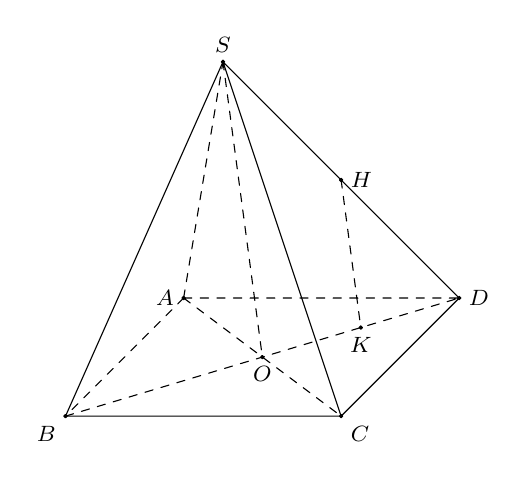
\begin{tikzpicture}[scale=0.5, font=\footnotesize, line join=round, line cap=round, >=stealth]
				\draw[fill=black] (0,0) node[left]{$A$} coordinate (A) circle(1.2pt);
				\draw[fill=black] (-3,-3) node[below left]{$B$} coordinate (B) circle(1.2pt);
				\draw[fill=black] (4,-3) node[below right]{$C$} coordinate (C) circle(1.2pt);
				\draw[fill=black] (7,0) node[right]{$D$} coordinate (D) circle(1.2pt);
				\draw[fill=black] (2,-1.5) node[below]{$O$} coordinate (O) circle(1.2pt);
				\draw[fill=black] (1,6) node[above]{$S$} coordinate (S) circle(1.2pt);
				\draw[fill=black] (4,3) node[right]{$H$} coordinate (H) circle(1.2pt);
				\draw[fill=black] (4.5, -0.75) node[below]{$K$} coordinate (K) circle(1.2pt);
				\draw[dashed] (A)--(S) (A)--(B) (A)--(C) (A)--(D) (B)--(D) (H)--(K) (S)--(O);
				\draw (S)--(B) (S)--(C) (S)--(D) (B)--(C)--(D);
		\end{tikzpicture}}
	}
\end{ex}
\begin{ex}%[1H4C1-4]%[Dự án D đợt 4 - Nguyễn Hoàng Anh]%[Đề ôn tập Chương IV - Khối 11 - Đề số 3]
	Cho hình chóp $S.A B C D$ có đáy là hình thang $A B C D$ với $A D \parallel B C$ và $A D=2 B C$. Gọi $M$ là điểm trên cạnh $S D$ thỏa $S M=\dfrac{1}{3} S D$. Mặt phẳng $(A B M)$ cắt cạnh bên $S C$ tại điểm $N$. Tính tỉ số $\dfrac{S N}{S C}$.
	\shortans{$0{,}5$}
	\loigiai{
		\begin{center}	
			\begin{tikzpicture}[scale=0.8,line width=0.7pt, font={\fontsize{12pt}{0pt}}, line join=round, line cap=round, >=stealth]
				%% Khai bao diem		
				\path
				(0,0) coordinate (B)
				(3,0) coordinate (C)
				(-1.5,1.4) coordinate (A)
				(5,1.4) coordinate (D) 
				(1.75,6) coordinate (S)
				($(S)!1/3!(D)$) coordinate (M)
				(intersection of C--D and A--B) coordinate (E)
				(intersection of S--C and M--E) coordinate (N)
				($(M)!2!(N)$) coordinate (K)
				;
				
				\draw (A)--(B) (C)--(D) (A)--(S)--(B) (K)--(C)--(S)--(D) (B)--(E)--(C) (S)--(E)--(M) ;
				\draw[dashed,line width=0.4pt] (B)--(C) (A)--(D) (A)--(M)--(B);
				%% vẽ điểm
				\foreach \x/\g in {A/180,B/200,C/-20,D/0,M/40,S/90,E/-90,N/10,K/160}
				\draw[fill=black] (\x) circle (.036)+(\g:.35)
				node{$\x$};	
				
			\end{tikzpicture}
		\end{center}
		Ta có $\heva{
			&  M \in (ABM)  \\
			&  M \in SD \subset (SCD)
		}$. Nên $M \in (ABM) \cap (SCD)$.\quad$(1)$\\[0.2cm]	
		Trong $(ABCD)$, gọi $E=AB \cap CD$.\\[0.2cm]
		Ta có $\heva{
			&  E \in AB \subset (ABM)  \\
			&  E \in CD \subset (SCD)
		}$. Nên $E \in (ABM) \cap (SCD)$.\quad$(2)$\\[0.2cm]
		Từ $(1)$ và $(2)$ suy ra $ME=(ABM) \cap (SCD)$.\\[0.2cm]
		Trong $(SCD)$, gọi $N=ME \cap SC$.\\[0.2cm]
		Khi đó $\heva{
			&  N \in SC  \\
			&  N \in ME \subset (ABM)
		}$. Suy ra $N=SC \cap (ABM)$.\\[0.2cm]
		Xét $\triangle AED$ có $BC \parallel AD$ nên $\dfrac{EC}{ED}=\dfrac{BC}{AD}=\dfrac{1}{2}$ (hệ quả Thales).\\[0.2cm]
		Mặt khác $SM=\dfrac{1}{3}SD=\dfrac{MS}{MD}=\dfrac{1}{2}$.\\[0.2cm]
		Trong $(SCD)$, kẻ $CK \parallel SD$ $(K \in EM)$.\\[0.2cm]
		Khi đó $\dfrac{CK}{MD}=\dfrac{EC}{ED}$ và $\dfrac{CK}{MS}=\dfrac{NC}{NS}$ (hệ quả Thales).\\[0.2cm]
		Suy ra $\dfrac{MD}{MS} \cdot \dfrac{NS}{NC} \cdot \dfrac{EC}{ED}=\dfrac{MD}{MS} \cdot \dfrac{MS}{CK} \cdot \dfrac{CK}{MD}=1$.\\[0.2cm]
		Do đó $\dfrac{NS}{NC}=\dfrac{ED}{EC} \cdot \dfrac{MS}{MD}=1$.\\[0.2cm]
		Vậy $\dfrac{SN}{SC}=\dfrac{1}{2}=0{,}5.$
	}
\end{ex}
\Closesolutionfile{ans}

\begin{center}
	\textbf{PHẦN 4 - TỰ LUẬN}
\end{center}
\begin{bt}%[1H4H3-3]%[1H4H1-4]%[Dự án D đợt 4 - Nguyễn Hoàng Anh]%[Đề ôn tập Chương IV - Khối 11 - Đề số 3]
	Cho hình chóp $S.ABCD$ có đáy là hình bình hành. Gọi $M$, $N$, $P$ lần lượt là trung điểm của các cạnh $BC$, $CD$, $SD$.
	\begin{enumerate}
		\item Xác định giao tuyến của hai mặt phẳng $(SAB)$ và $(SCD)$.
		\item Tìm giao điểm $H$ của $BP$ và mặt phẳng $(SAC)$.
		\item Chứng minh rằng $NP\parallel(SBC)$.
		\item Gọi $Q$ là giao điểm của $SA$ với $(MNP)$. Tính tỉ số $\dfrac{SQ}{SA}$.
	\end{enumerate}
	\loigiai{
		\begin{center}
			\begin{tikzpicture}[font=\footnotesize, line join=round, line cap=round, >=stealth,scale=1]
				\path
				(0,0) coordinate (A) 
				(-2,-2) coordinate (B)
				(3,-2) coordinate (C)
				(5,0) coordinate (D)
				(0.5,4) coordinate (S)
				($(A)!.5!(C)$) coordinate (O)
				($(B)!.5!(C)$) coordinate (M)
				($(C)!.5!(D)$) coordinate (N)
				($(D)!.5!(S)$) coordinate (P)
				($(S)!.25!(A)$) coordinate (Q)
				(intersection of M--N and A--C) coordinate (I)
				(intersection of S--O and B--P) coordinate (H)
				;
				\draw 
				(S)--(B)--(C)--(D)--cycle
				(S)--(C) (N)--(P);
				\draw [dashed] (S)--(A)--(D)--(B)--(A)--(C) (I)--(Q) (P)--(M)--(N) (M)--(Q)--(P)--(B) (S)--(O);
				\draw (-2,1.5)--(2,5.5)node[above]{$d$};
				\foreach \x/\g in
				{A/150,B/180,C/0,D/0,S/90,O/-90,M/-90,N/0,P/60,I/-90,Q/220,H/180}
				\fill[black](\x) circle (1pt)
				($(\x)+(\g:3mm)$) node{$\x$};
			\end{tikzpicture}		
		\end{center}
		\begin{enumerate}
			\item Ta có 
			$\heva{& AB \subset(SAB) \\& CD\subset(SCD)\\&AB\parallel CD\\&S \in(SAB) \cap(SCD)}$.\\
			Vậy $d$ là giao tuyến của hai mặt phẳng $(SAB)$ và $(SCD)$ với $d\parallel AB\parallel CD$, $S \in d$.
			\item Trong mặt phẳng $(ABCD)$,
			gọi $O=AC \cap BD$.\\
			Suy ra $SO=(SAC) \cap(SBD)$.\\
			Trong mặt phẳng $(SBD)$, gọi $H=BP \cap SO$.\\
			Vậy $BP \cap(SAC)=H$.
			\item Vì $P$, $N$ lần lượt là trung điểm của $SD$, $CD$ nên $NP$ là đường trung bình của tam giác $SCD$.\\
			Suy ra $NP\parallel SC$.\\
			Mà $SC \subset(SBC)$ nên $NP\parallel(SBC)$.
			\item Trong mặt phẳng $(ABCD)$, gọi $I$ là giao điểm của $AC$ và $MN$.\\
			Trong mặt phẳng $(SAC)$, lấy $Q$ thuộc $SA$ sao cho $IQ\parallel SC$.\\
			Khi đó, ta có $I\in(MNP)$ và $IQ\parallel NP$ nên $Q\in(MNP)$.\\
			Vậy $Q$ là giao điểm của $SA$ với mặt phẳng $(MNP)$.\\
			Ta có $MN$ là đường trung bình của tam giác $BCD$ nên $MN\parallel BD$ hay $NI\parallel DO$.\\
			Trong tam giác $DOC$ có $NI\parallel DO$ và $N$ là trung điểm của $CD$ nên $NI$ là đường trung bình của tam giác $DOC$, suy ra $I$ là trung điểm của $OC$.\\
			Khi đó $\dfrac{CI}{CO}=\dfrac{1}{2}\Rightarrow \dfrac{CI}{CA}=\dfrac{1}{4}$.\\
			Xét tam giác $SAC$, ta có $IQ\parallel SC$ nên $\dfrac{SQ}{SA}=\dfrac{CI}{CA}=\dfrac{1}{4}$.
		\end{enumerate}		
	}
\end{bt}

\begin{bt}%[1H4V4-6]%[Dự án D đợt 4 - Nguyễn Hoàng Anh]%[Đề ôn tập Chương IV - Khối 11 - Đề số 3]
	Cho hình chóp $S.ABCD$ có đáy $ABCD$ là hình bình hành tâm $O$. Lấy $M$ trên cạnh $SA$ sao cho $MA=2MS$, $N$ trên cạnh $BC$ sao cho $NB=2NC$ và $G$ là trọng tâm tam giác $BCD$.
	\begin{enumerate}
		\item Tìm giao tuyến của hai mặt phẳng $(SAD)$ và $(MBC)$.
		\item Chứng minh $(MNG)$ song song với $(SCD)$.
		\item Cho biết tam giác $SCD$ vuông tại $S$ có $SC=3$, $SD=4$. Tính tỉ số $\dfrac{MN}{AB}$.
	\end{enumerate}
	\loigiai{
		\begin{enumerate}
			\immini{
				\item Ta có $\heva{&M\in (SAD)\cap (MBC)\\ &AD \parallel BC\\ &AD\subset (SAD),\, BC\subset (MBC).}$\\
				Suy ra $(SAD)\cap (MBC)=d$ với $d$ qua $M$ và song song với $AD$, $BC$.
				\item Vì $G$ là trọng tâm của tam giác $BCD$.\\
				Nên $CG=\dfrac{2}{3}CO=\dfrac{1}{3}CA\Rightarrow CG=\dfrac{1}{2}AG$.\\
				Xét $\triangle SAC$ có $\dfrac{MA}{MS}=\dfrac{GA}{GC}=2$.\\
				Suy ra $MG\parallel SC $ (định lí Thales đảo).\\
				Xét $\triangle ABC$ có $\dfrac{NB}{NC}=\dfrac{GA}{GC}=2$.\\
				Suy ra $NG\parallel AB$ (định lí Thales đảo).\\
				Mà $AB \parallel CD $.
				Do đó $NG\parallel CD$.\\
				Ta có $\heva{&MG\parallel SC \, \text{(cmt)}\\&NG\parallel CD \, \text{(cmt)} \\ &MG,\, NG \subset (MNG)\\ &SC,\, CD\subset (SCD).}$\\
				Suy ra $(MNG)\parallel (SCD)$.}
			{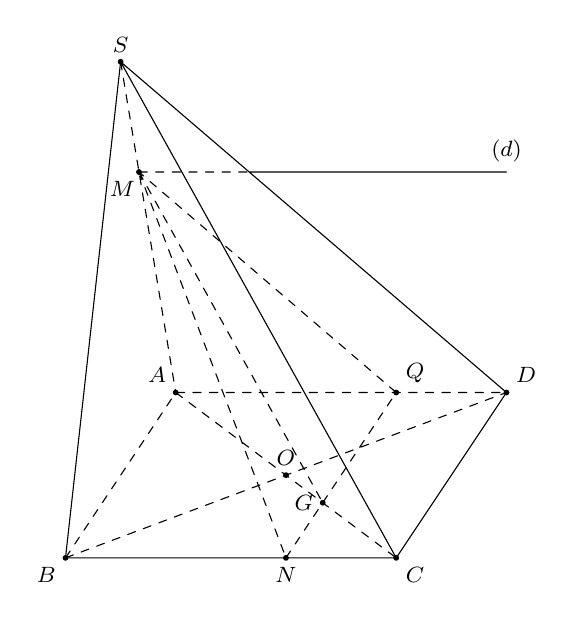
\begin{tikzpicture}[scale=0.7, font=\footnotesize, line join=round, line cap=round, >=stealth]
					\draw[fill=black] (0,0) node[above left]{$A$} coordinate (A) circle(1.2pt);
					\draw[fill=black] (-2,-3) node[below left]{$B$} coordinate (B) circle(1.2pt);
					\draw[fill=black] (4,-3) node[below right]{$C$} coordinate (C) circle(1.2pt);
					\draw[fill=black] (6,0) node[above right]{$D$} coordinate (D) circle(1.2pt);
					\draw[fill=black] (-1,6) node[above]{$S$} coordinate (S) circle(1.2pt);
					\draw[fill=black] (2,-1.5) node[above]{$O$} coordinate (O) circle(1.2pt);
					\draw[fill=black] (2,-3) node[below]{$N$} coordinate (N) circle(1.2pt);
					\draw[fill=black] (4,0) node[above right]{$Q$} coordinate (Q) circle(1.2pt);
					\draw[fill=black] (8/3,-2) node[left]{$G$} coordinate (G) circle(1.2pt);
					\draw[fill=black] (-2/3,4) node[below, xshift=-6pt]{$M$} coordinate (M) circle(1.2pt);
					\draw[fill=black] (4/3,4) coordinate (M');
					\draw[fill=black] (6,4) node[above]{$(d)$} coordinate (d);
					\draw (S)--(B) (S)--(B) (S)--(C) (S)--(D) (B)--(C)--(D) (M')--(d);
					\draw[dashed] (A)--(C) (B)--(D) (S)--(A) (B)--(A)--(D) (N)--(Q)--(M) (M)--(M') (M)--(N) (M)--(G);
				\end{tikzpicture}
			}
			\item Ta có $AB=CD=\sqrt{SC^2 + SD^2}=5$.\\
			Vì $\heva{&(MNG)\parallel (SCD)\\ &(SAD)\cap (SCD)=SD.}$\\
			Nên $(SAD)\cap (MNG)= MQ\parallel SD $ ($Q\in AD$).\\
			Suy ra $\dfrac{MQ}{SD}=\dfrac{AM}{AS}=\dfrac{2}{3} \Rightarrow MQ=\dfrac{2}{3}SD=\dfrac{8}{3}$.\\
			Ta có $\heva{&MG=\dfrac{2}{3}SC=\dfrac{2}{3}\cdot 3 =2 \\ &GQ=\dfrac{2}{3}CD = \dfrac{2}{3}\cdot 5 = \dfrac{10}{3}\\ & MQ=\dfrac{8}{3}.}$\\
			Suy ra $MG^2 + MQ^2 = GQ^2$.\\
			Do đó $\triangle MGQ$ vuông tại $M$.\\
			Khi đó $\cos \left( \widehat{MQN} \right) =\dfrac{MQ}{GQ}=\dfrac{4}{5}$.\\
			Áp dụng định lí cosin cho tam giác $MNQ$ ta có
			\begin{align*}
				MN^2 &= QM^2 + QN^2 - 2\cdot QM \cdot QN \cdot \cos \left(\widehat{MQN} \right)\\
				&= \left(\dfrac{8}{3} \right)^2 + 5^2 - 2\cdot \dfrac{8}{3}\cdot 5\cdot \dfrac{4}{5}\\
				&= \dfrac{97}{5}.
			\end{align*}
			Do đó $MN=\dfrac{\sqrt{97}}{3}$. Suy ra $\dfrac{MN}{AB}=\dfrac{\sqrt{97}}{15}$.
		\end{enumerate}
	}
\end{bt}
\begin{bt}%[1H4V4-7]%[1H4V4-4]%[Dự án D đợt 4 - Nguyễn Hoàng Anh]%[Đề ôn tập Chương IV - Khối 11 - Đề số 3]
	Nhà bạn Lan có một đèn trang trí khung hình chóp tam giác $S.ABC$. Vị trí bóng đèn tiếp xúc với mặt đáy $(ABC)$ tại trọng tâm $G$ của tam giác $ABC$. Mẹ Lan nhờ Lan xác định vị trí điểm $M$ trên cạnh $SA$ của đèn. Biết rằng $M$ là giao điểm của $SA$ với mặt phẳng $(\alpha)$, và mặt phẳng
	$(\alpha)$ đi qua $G$ và song song với mặt phẳng $(SBC)$. Em hãy giúp Lan tính tỉ số $\dfrac{SM}{AM}$.
	\begin{center}
	\begin{minipage}[t]{0.45\textwidth}
		
\begin{tikzpicture}[line cap=round,line join=round]
			\path[draw=gray, fill] (0, 6) -- (-0.08, 6) -- (-0.08, 5.22) -- (-0.15, 5.18) --
			(-0.15, 4.96) .. controls +(0:0) and +(90:0.04) ..
			(-0.23, 4.89) .. controls +(-90:0.04) and +(0:0) ..
			(-0.19, 4.81) -- (-0.19, 4.43) -- (-0.56, 3.45) .. controls +(0:0) and +(89:0.36) ..
			(-0.56, 2.38) -- (0.52, 2.38) .. controls +(91:0.36) and +(0:0) ..
			(0.52, 3.45) -- (0.15, 4.43) -- (0.15, 4.81) .. controls +(0:0) and +(-90:0.04) ..
			(0.19, 4.89) .. controls +(90:0.04) and +(0:0) ..
			(0.11, 4.96) -- (0.11, 5.18) -- (0.04, 5.22) -- (0.04, 6) --
			(-0.04, 6);
			
			\def\bongden{(-0, -0.21) .. controls +(178:0.68) and +(-88:0.82) ..
				(-1.24, 1.1) .. controls +(92:0.32) and +(-160:0.5) ..
				(-0.56, 2.06) .. controls +(53:0.07) and +(-81:0.07) ..
				(-0.48, 2.23) .. controls +(96:0.07) and +(-90:0.04) ..
				(-0.56, 2.38) .. controls +(13:0.36) and +(168:0.36) ..
				(0.52, 2.38) .. controls +(-90:0.04) and +(84:0.07) ..
				(0.44, 2.23) .. controls +(-96:0.07) and +(127:0.07) ..
				(0.52, 2.06) .. controls +(-20:0.5) and +(89:0.32) ..
				(1.2, 1.1) .. controls +(-92:0.82) and +(2:0.68) ..
				(-0.04, -0.21);}
			
			\path[inner color=orange, outer color=yellow] \bongden
			
			\path[top color=black, bottom color=gray, even odd rule]
			(-3.62, 0) -- (-0.38, -1.06) -- (3.5, 0) --cycle
			(-1.39, -0.24) -- (-0.59, -0.51) -- (-0.58, -0.24) --cycle
			(-0.06, -0.24) -- (-0.05, -0.55) -- (1.09, -0.25) --cycle;
			
			\path[top color=black, bottom color=gray!35!black, even odd rule]
			(-0.3, 4.67) -- (-3.62, 0) -- (3.5, 0) -- (0.26, 4.67) --cycle
			(0.05, 4.27) -- (-0.1, 4.27) -- (-2.84, 0.41) -- (2.73, 0.41) --cycle;
		\end{tikzpicture}
	\end{minipage}
	\begin{minipage}[t]{0.45\textwidth}
		\begin{tikzpicture}[line join = round, line cap = round,>=stealth,font=\footnotesize,scale=1,declare function={ac=5;ab=2.2; gocB=-60;ha=3.5;}]
			\path 
			(0,0) coordinate (A)
			(ac,0) coordinate (C)
			(gocB:ab) coordinate (B)
			($(B)!0.5!(C)$) coordinate (BC)
			($(A)!0.5!(B)$) coordinate (AB)
			(intersection of C--AB and A--BC) coordinate (G)
			($(G)+(0,ha)$) coordinate (S);
			\draw (S)--(A)--(B)--(C)--cycle (S)--(B);
			\draw[dashed] (A)--(C);
			\foreach \x/\gm in {S/90,A/180,B/-90,C/0,G/-90} \fill (\x) circle (1pt) ($(\x)+(\gm:3.5mm)$)node{$\x$};
		\end{tikzpicture}	
	\end{minipage}
\end{center}
	\loigiai{
		\begin{center}
			\begin{tikzpicture}[line join = round, line cap = round,>=stealth,font=\footnotesize,scale=1,declare function={ac=5;ab=2.2; gocB=-60;ha=3.5;}]
				\path 
				(0,0) coordinate (A)
				(ac,0) coordinate (C)
				(gocB:ab) coordinate (B)
				($(B)!0.5!(C)$) coordinate (BC)
				($(A)!0.5!(B)$) coordinate (AB)
				(intersection of C--AB and A--BC) coordinate (G)
				($(G)+(0,ha)$) coordinate (S)
				($(A)!2/3!(B)$) coordinate (N)
				($(A)!2/3!(C)$) coordinate (P)
				($(A)!2/3!(S)$) coordinate (M)
				;
				\draw (S)--(A)--(B)--(C)--cycle (S)--(B) (M)--(N);
				\draw[dashed] (A)--(C) (M)--(P)--(N);
				\foreach \x/\gm in {S/90,A/180,B/-90,C/0,G/-90,N/-150,M/150,P/70} \fill (\x) circle (1pt) ($(\x)+(\gm:3.5mm)$)node{$\x$};
			\end{tikzpicture}		
		\end{center}
		Trong mặt phẳng $(ABC)$: Qua $G$ kẻ đường thẳng song song $BC$ cắt $AB$ và $AC$ lần lượt tại $N$ và $P$.\\
		Trong mặt phẳng $(SAC)$: Qua $P$ kẻ đường thẳng song song $SC$ cắt $SA$ tại $M$.\\
		Ta có $\heva{& NP\parallel BC \\ & PN\parallel SC \\ & SC\subset (SBC) \\ & BC\subset (SBC) \\ & MP\cap NP=\{P\}}\Rightarrow \left(MNP\right)\parallel\left(SBC\right)$.\\
		$M$ là giao điểm của $\left(\alpha\right)$ với $SA$ suy ra $SA\cap(MNP)=\{M\}$.\\
		Vì $NP\parallel BC$ nên theo định lý Thales ta có $\dfrac{AG}{AD}=\dfrac{AN}{AB}=\dfrac{AP}{AC}=\dfrac{2}{3}$.\\
		$MP\parallel SC$ nên theo định lý Thales ta có $\dfrac{SM}{AM}=\dfrac{CP}{AP}=\dfrac{1}{2}$.
	}
\end{bt}
